\documentclass[a4paper]{article}

\usepackage{fullpage}

\usepackage{graphicx}
\usepackage{caption}
\usepackage{subcaption}

\usepackage{amsmath}

% Code for typesttting C code
\usepackage{listings}
\usepackage{color}

\definecolor{mygreen}{rgb}{0,0.6,0}
\definecolor{mygray}{rgb}{0.5,0.5,0.5}
\definecolor{mymauve}{rgb}{0.58,0,0.82}
\definecolor{mybrown}{rgb}{0.5,0,0}

\lstdefinestyle{MyCStyle}{ %
  language=C,                      % the language of the code
  backgroundcolor=\color{white},   % choose the background color; you must add \usepackage{color} or \usepackage{xcolor}
  basicstyle=\ttfamily    ,        % the size of the fonts that are used for the code
  breakatwhitespace=false,         % sets if automatic breaks should only happen at whitespace
  breaklines=true,                 % sets automatic line breaking
  captionpos=b,                    % sets the caption-position to bottom
  commentstyle=\color{mygreen},    % comment style
  deletekeywords={...},            % if you want to delete keywords from the given language
  escapeinside={\%*}{*)},          % if you want to add LaTeX within your code
  extendedchars=true,              % lets you use non-ASCII characters; for 8-bits encodings only, does not work with UTF-8
  frame=single,                    % adds a frame around the code
  keepspaces=true,                 % keeps spaces in text, useful for keeping indentation of code (possibly needs columns=flexible)
  keywordstyle=\color{blue},       % keyword style
  morecomment=[l][\color{mybrown}]\#,  % compiler directive
  morekeywords={*,...},            % if you want to add more keywords to the set
  numbers=left,                    % where to put the line-numbers; possible values are (none, left, right)
  numbersep=5pt,                   % how far the line-numbers are from the code
  numberstyle=\tiny\color{mygray}, % the style that is used for the line-numbers
  rulecolor=\color{black},         % if not set, the frame-color may be changed on line-breaks within not-black text (e.g. comments (green here))
  showspaces=false,                % show spaces everywhere adding particular underscores; it overrides 'showstringspaces'
  showstringspaces=false,          % underline spaces within strings only
  showtabs=false,                  % show tabs within strings adding particular underscores
  stepnumber=1,                    % the step between two line-numbers. If it's 1, each line will be numbered
  stringstyle=\color{mymauve},     % string literal style
  tabsize=2,                       % sets default tabsize to 2 spaces
  title=\lstname                   % show the filename of files included with \lstinputlisting; also try caption instead of title
}

\lstdefinestyle{MyASMStyle}{ %
  language=[x86masm]Assembler,     % the language of the code
  backgroundcolor=\color{white},   % choose the background color; you must add \usepackage{color} or \usepackage{xcolor}
  basicstyle=\ttfamily    ,        % the size of the fonts that are used for the code
  breakatwhitespace=false,         % sets if automatic breaks should only happen at whitespace
  breaklines=true,                 % sets automatic line breaking
  captionpos=b,                    % sets the caption-position to bottom
  commentstyle=\color{mygreen},    % comment style
  deletekeywords={...},            % if you want to delete keywords from the given language
  escapeinside={\%*}{*)},          % if you want to add LaTeX within your code
  extendedchars=true,              % lets you use non-ASCII characters; for 8-bits encodings only, does not work with UTF-8
  frame=single,                    % adds a frame around the code
  keepspaces=true,                 % keeps spaces in text, useful for keeping indentation of code (possibly needs columns=flexible)
  keywordstyle=\color{blue},       % keyword style
  morecomment=[l][\color{mybrown}]\#,  % compiler directive
  morekeywords={*,...},            % if you want to add more keywords to the set
  numbers=left,                    % where to put the line-numbers; possible values are (none, left, right)
  numbersep=5pt,                   % how far the line-numbers are from the code
  numberstyle=\tiny\color{mygray}, % the style that is used for the line-numbers
  rulecolor=\color{black},         % if not set, the frame-color may be changed on line-breaks within not-black text (e.g. comments (green here))
  showspaces=false,                % show spaces everywhere adding particular underscores; it overrides 'showstringspaces'
  showstringspaces=false,          % underline spaces within strings only
  showtabs=false,                  % show tabs within strings adding particular underscores
  stepnumber=1,                    % the step between two line-numbers. If it's 1, each line will be numbered
  stringstyle=\color{mymauve},     % string literal style
  tabsize=2,                       % sets default tabsize to 2 spaces
  title=\lstname                   % show the filename of files included with \lstinputlisting; also try caption instead of title
}

\newlength{\pic}

\begin{document}

\title{EE445M Lab 3 Report}
\author{Yen-Kai Huang \\ Siavash Zanganeh Kamali}
\maketitle

\section{Objective} The goal of this lab is to extend the RTOS we built in Lab1 and Lab2 to include blocking and priority scheduling. We will also extend the RTOS to include two real-time periodic tasks, two aperiodic button tasks, and minimally invasive tools to carry out performance measures. The interpreter will be extended to allow recording debugging/performance data and downloading them to the PC screen through UART. 

\section{Software Design}
In this lab we implemented priority scheduler, and blocking semaphore. Implementing priority scheduler requires
rewriting all the functions that deal with the thread link-list structures (\textbf{AddThread}, \textbf{wake-up
background thread}, \textbf{Signal}, \textbf{Kill}, \textbf{Sleep}, \textbf{Block})

\lstset{language=C, style=MyCStyle}
\lstinputlisting{Code/OS.c}

The change does not involve osasm.c

\lstset{language=C, style=MyASMStyle}
\lstinputlisting{Code/osasm.s}

Then we test the blocking semaphore with this program.

\lstset{language=C, style=MyCStyle}
\lstinputlisting{Code/Testmain3_blocking.c}

We also measured the jitter with this program.

\lstset{language=C, style=MyCStyle}
\lstinputlisting{Code/Jitter_measurement.c}

\section{Measurement}

\paragraph{(a) Plot of the logic analyzerrunning the blocking/sleeping/killing/round-robin system\\}

We imitate a round-robin system by setting all the priorities of threads (T1, T2, T3) to an equal value.
Background thread S1 and S2 are signalling until a counter counts to a threshold value. And foreground
thread ST signals until it kills itself. See Figure-\ref{RR}.

\setlength{\pic}{0.8\textwidth}

\begin{figure}[htp]
\center
	\begin{subfigure}[H]{\pic}
	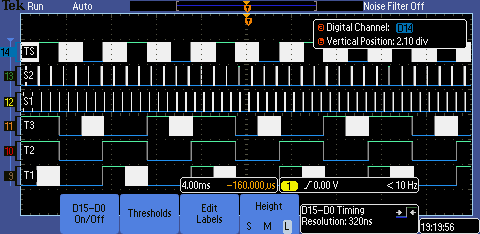
\includegraphics[width=\pic]{Scope/RR_a}
	\caption{Initial execution}
	\end{subfigure}
	\\[5pt]
	\begin{subfigure}[H]{\pic}
	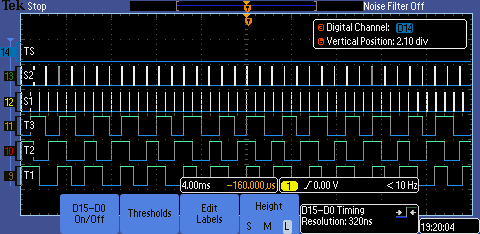
\includegraphics[width=\pic]{Scope/RR_b}
	\caption{After ST kills itself}
	\end{subfigure}
	\\[5pt]
	\begin{subfigure}[H]{\pic}
	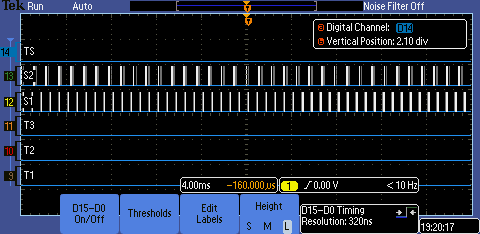
\includegraphics[width=\pic]{Scope/RR_c}
	\caption{After the signalling stops}
	\end{subfigure}
	
\caption{Scope showing Round-robin scheduler running}
\label{RR}
\end{figure}

\paragraph{(b) Plot of the scope window running the blocking/sleeping/killing/priority system \\}

Figure-\ref{PRI} shows the scope picture of running a priority scheduler on the Producer-Consumer main.
The labels show the name of the threads. Among those, DAS is a periodic background thread, all the other threads
are foreground threads. Button is an aperiodic thread caused by pressing the switch. The Interpreter thread is
a foreground thread that waits on user input, therefore also aperiodic.

\setlength{\pic}{0.8\textwidth}

\begin{figure}[htp]
\center
	\begin{subfigure}[H]{\pic}
	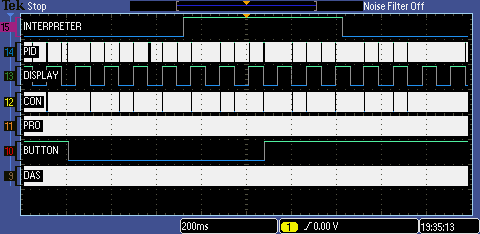
\includegraphics[width=\pic]{Scope/Pri}
	\caption{Initial execution}
	\end{subfigure}
	\\[5pt]
	\begin{subfigure}[H]{\pic}
	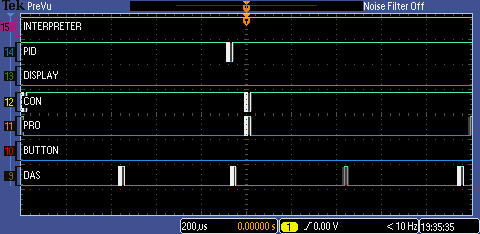
\includegraphics[width=\pic]{Scope/Pri_zoom}
	\caption{Zoomed-in picture}
	\end{subfigure}
\caption{Scope showing Priority scheduler running}
\label{PRI}
\end{figure}

\paragraph{(c) Table like Table 3.1 each showing performance measurements versus sizes of
the Fifo and timeslices. \\}
See Table-1.

\begin{center}
\begin{tabular}{|l|l|l|l|l|}
\hline
\multicolumn{5}{|c|}{Performance Measurement} \\
\hline
\multicolumn{5}{|c|}{Spinlock/Non-Cooperative} \\
\hline
FIFOSize  &  TIMESLICE(ms)  &  DataLost  &  Jitter($\mu s$)  &  PIDWork\\
\hline
4  &  2  &  1895  &  9  &  1842\\
8  &  2  &  0  &  9  &  1743\\
32  &  2  &  0  &  9  &  1743\\
32  &  1  &  0  &  10  &  1745\\
32  &  10  &  0  &  9  &  1778\\
\hline
\multicolumn{5}{|c|}{Spinlock/Cooperative} \\
\hline
FIFOSize  &  TIMESLICE(ms)  &  DataLost  &  Jitter($\mu s$)  &  PIDWork\\
\hline
4  &  2  &  1916  &  10  &  2656\\
8  &  2  &  0  &  9  &  2507\\
32  &  2  &  0  &  10  &  2507\\
32  &  1  &  0  &  10  &  2507\\
32  &  10  &  0  &  9  &  2510\\
\hline
\multicolumn{5}{|c|}{Block/Priority} \\
\hline
FIFOSize  &  TIMESLICE(ms)  &  DataLost  &  Jitter($\mu s$)  &  PIDWork\\
\hline
4  &  2  &  1473  &  1  &  5388\\
8  &  2  &  986  &  1  &  5316\\
32  &  2  &  0  &  1  &  5153\\
32  &  1  &  0  &  1  &  5153\\
32  &  10  &  0  &  1  &  5153 \\
\hline
\end{tabular}
\label{PM}\\
\textbf{Table 1.\ Performance Measurements}
\end{center}

\section{Analysis and Discussion}
\paragraph{How would your implementation of OS\_AddPeriodicThread be different if there were 10 background
threads? (Preparation 1)\\}

Instead of using different timers for each background thread, use one background thread that runs all the other threads. For each background thread, there should be a data structure that holds a pointer to the background function, the period of the thread, and the current time remaining to next execution. (In units of the period of the
timer interrupt) The interrupt will pass through each thread, decrements their counter, execute if the counter is 0, and then sets their timer to the reload value again. This can work for any number of periodic tasks.
 
\paragraph{How would your implementation of blocking semaphores be different if there were 100 foreground threads?
(Preparation 4) \\}

Since we are using linking and unlinking, our implementation is functional if there were 100 foreground threads.
The scheduler is as fast as a scheduler without blocking semaphores. The only limitation will be the heap space
in our dynamic memory allocation module.
 
\paragraph{How would your implementation of the priority scheduler be different if there were 100 foreground
threads?  (Preparation 5) \\}

Since we're using different linked list for every priority, our implementation is compatible with 100 foreground threads. However, if the number of  priority levels increases, a better method of searching should be implemented rather than a simple linear search to find the available highest priority.
 
\paragraph{What happens to your OS if all the threads are blocked? If your OS would crash, describe exactly what the 
OS does? What happens to your OS if all the threads are sleeping? If your OS would crash, describe exactly 
what the OS does? If you answered crash to either or both, explain how you might change your OS to prevent 
the crash. \\}

If last active thread blocks, the scheduler assigns the last thread to be blocked as the next thread to be run, and therefore the OS continues running the foreground thread that was supposed to be blocked. This is an unexpected behaviour and will probably cause a crash in the system.

If last active thread sleeps, the scheduler assigns the last thread to be slept as the next thread to be run, and therefore the OS continues running the foreground threads that were supposed to be asleep. This can cause undefined behaviour and eventually crash the system.

Currently, our OS\_Init always adds a dummy thread at the lowest priority that will always remain active which prevents crashes. a more robust method will be to make the microcontroller sleeps in case of no active foreground thread and waits for interrupts to occur.
 
\paragraph{What happens to your OS if one of the foreground threads returns? e.g., what if you added this
foreground\\[5pt] } 

\begin{quote}
\vspace{-25pt}
\lstset{language=C, frame=none, numbers=none}
\begin{lstlisting}
void BadThread(void){ int i; 
 	for(i=0; i<100; i++){}; 
 	return; 
}
\end{lstlisting}
\end{quote}
\vspace{-30pt}
\textbf{What should your OS have done in this case? Do not implement it, rather, with one sentence, say what the OS 
should have done? Hint: I asked this question on an exam. }

OS should have detected that a foreground thread has tried to return and therefore killed the faulty thread.
 
\paragraph{What are the advantages of spinlock semaphores over blocking semaphores? What are the advantages of 
blocking semaphores over spinlock? \\}
 
Spinlock semaphores are easier to implement and do not slow down the process of choosing next thread in the scheduler. However, blocking semaphores can be a lot faster, more CPU efficient, and can provide the means to implement bounded waiting.
 
\paragraph{Consider the case where thread $T_1$ interrupts thread $T_2$, and we are experimentally verifying the 
system operates without critical sections. Let \emph{n} be the number of times $T_1$ interrupts $T_2$. Let 
\emph{m} be the total number of interruptible locations within  $T_2$. Assume the time during which $T_1$ triggers 
is random with respect to the place (between which two instructions of  $T_2$) it gets interrupted. In other words, 
there are \emph{m} equally-likely places within $T_2$ for the $T_1$ interrupt to occur. What is the probability 
after \emph{n} interrupts that a particular place in  $T_2$ was never selected? Furthermore, what is the 
probability that all locations were interrupted at least once?\\}

Probability that a line was never selected is $(m-1/m) ^ n$ \\
Probability that all locations were interrupted once
\begin{equation*}
p =
\begin{cases}
  0                                            &\mbox{if } n < m \\
  \left( 1-\left(\frac{m-1}{m} \right)^n \right)^m         &\mbox{if } n \ge m
\end{cases}
\end{equation*}


\end{document}